\documentclass[14pt]{extbook}
\usepackage{multicol, enumerate, enumitem, hyperref, color, soul, setspace, parskip, fancyhdr} %General Packages
\usepackage{amssymb, amsthm, amsmath, latexsym, units, mathtools} %Math Packages
\everymath{\displaystyle} %All math in Display Style
% Packages with additional options
\usepackage[headsep=0.5cm,headheight=12pt, left=1 in,right= 1 in,top= 1 in,bottom= 1 in]{geometry}
\usepackage[usenames,dvipsnames]{xcolor}
\usepackage{dashrule}  % Package to use the command below to create lines between items
\newcommand{\litem}[1]{\item#1\hspace*{-1cm}\rule{\textwidth}{0.4pt}}
\pagestyle{fancy}
\lhead{Progress Quiz 2}
\chead{}
\rhead{Version B}
\lfoot{4389-3341}
\cfoot{}
\rfoot{Summer C 2021}
\begin{document}

\begin{enumerate}
\litem{
Solve the quadratic equation below. Then, choose the intervals that the solutions belong to, with $x_1 \leq x_2$ (if they exist).\[ 19x^{2} +11 x -9 = 0 \]\begin{enumerate}[label=\Alph*.]
\item \( x_1 \in [-0.6, -0.08] \text{ and } x_2 \in [0.9, 1.11] \)
\item \( x_1 \in [-1.65, -0.82] \text{ and } x_2 \in [0.27, 0.99] \)
\item \( x_1 \in [-20.06, -18.74] \text{ and } x_2 \in [8.64, 8.73] \)
\item \( x_1 \in [-28.81, -27.69] \text{ and } x_2 \in [27.6, 28.12] \)
\item \( \text{There are no Real solutions.} \)

\end{enumerate} }
\litem{
Factor the quadratic below. Then, choose the intervals that contain the constants in the form $(ax+b)(cx+d); b \leq d.$\[ 24x^{2} +38 x + 15 \]\begin{enumerate}[label=\Alph*.]
\item \( a \in [0.6, 1.5], \hspace*{5mm} b \in [11, 20], \hspace*{5mm} c \in [0.4, 2.5], \text{ and } \hspace*{5mm} d \in [16, 27] \)
\item \( a \in [3.6, 7.6], \hspace*{5mm} b \in [0, 7], \hspace*{5mm} c \in [4.5, 8.6], \text{ and } \hspace*{5mm} d \in [3, 7] \)
\item \( a \in [0.6, 1.5], \hspace*{5mm} b \in [0, 7], \hspace*{5mm} c \in [17.3, 20.6], \text{ and } \hspace*{5mm} d \in [3, 7] \)
\item \( a \in [7.3, 10], \hspace*{5mm} b \in [0, 7], \hspace*{5mm} c \in [2.1, 4.4], \text{ and } \hspace*{5mm} d \in [3, 7] \)
\item \( \text{None of the above.} \)

\end{enumerate} }
\litem{
Graph the equation below.\[ f(x) = (x+2)^2 - 13 \]\begin{enumerate}[label=\Alph*.]
\begin{multicols}{2}\item 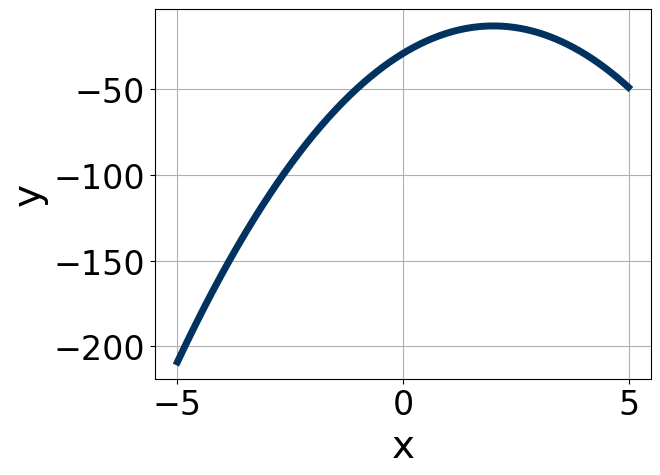
\includegraphics[width = 0.3\textwidth]{../Figures/quadraticEquationToGraphCopyAB.png}\item 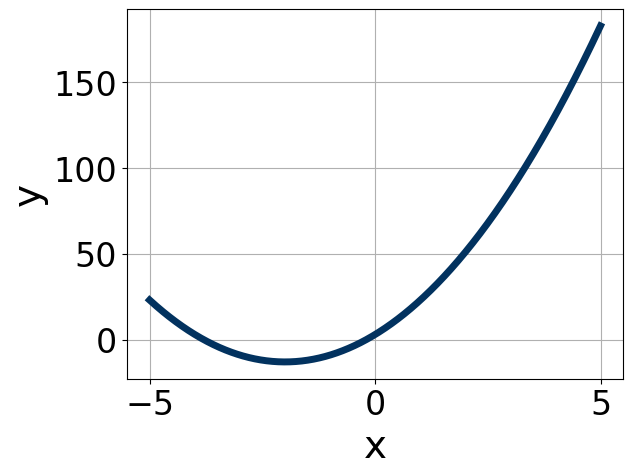
\includegraphics[width = 0.3\textwidth]{../Figures/quadraticEquationToGraphCopyBB.png}\item 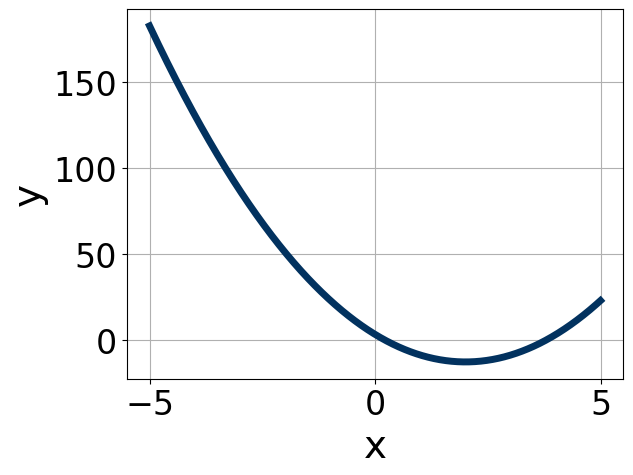
\includegraphics[width = 0.3\textwidth]{../Figures/quadraticEquationToGraphCopyCB.png}\item 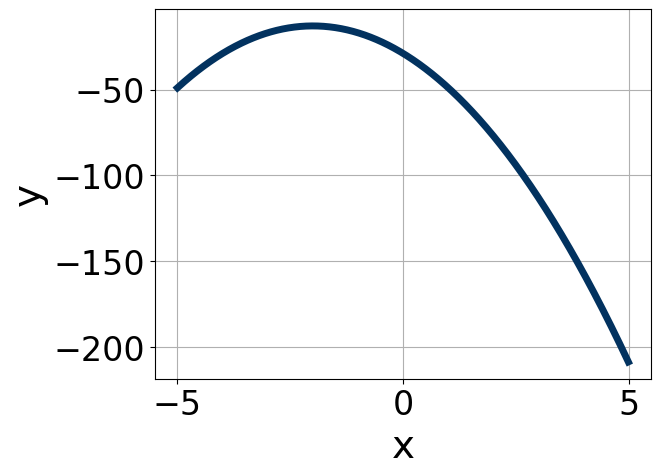
\includegraphics[width = 0.3\textwidth]{../Figures/quadraticEquationToGraphCopyDB.png}\end{multicols}\item None of the above.
\end{enumerate} }
\litem{
Graph the equation below.\[ f(x) = -(x-3)^2 + 12 \]\begin{enumerate}[label=\Alph*.]
\begin{multicols}{2}\item 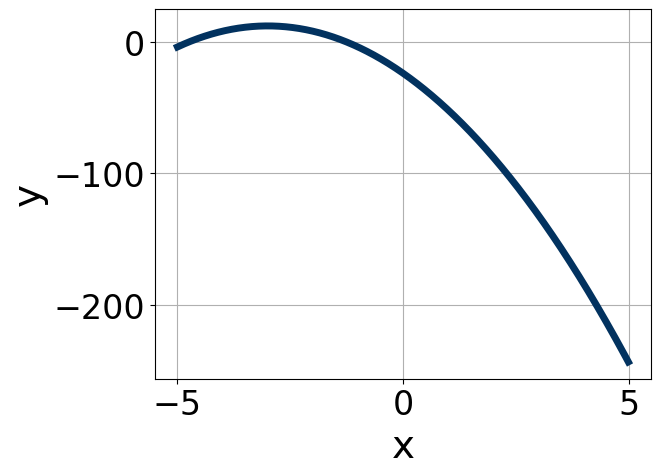
\includegraphics[width = 0.3\textwidth]{../Figures/quadraticEquationToGraphAB.png}\item 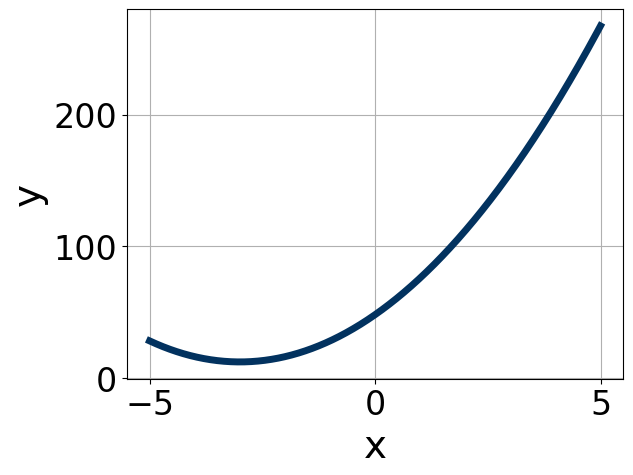
\includegraphics[width = 0.3\textwidth]{../Figures/quadraticEquationToGraphBB.png}\item 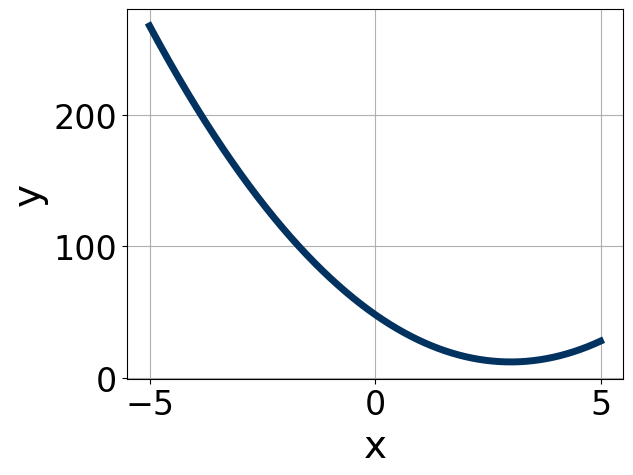
\includegraphics[width = 0.3\textwidth]{../Figures/quadraticEquationToGraphCB.png}\item 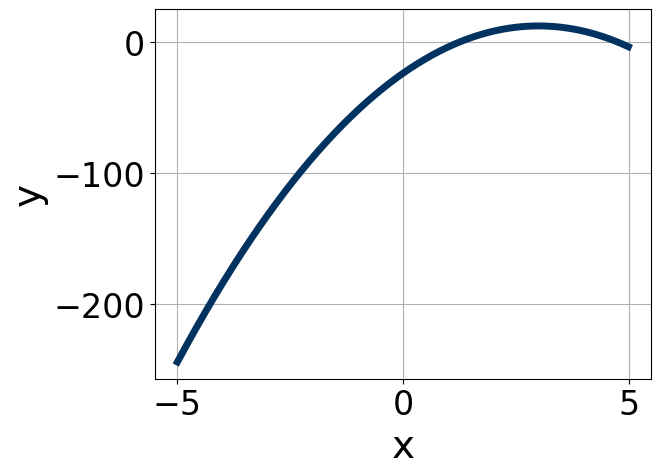
\includegraphics[width = 0.3\textwidth]{../Figures/quadraticEquationToGraphDB.png}\end{multicols}\item None of the above.
\end{enumerate} }
\litem{
Solve the quadratic equation below. Then, choose the intervals that the solutions belong to, with $x_1 \leq x_2$ (if they exist).\[ -18x^{2} +8 x + 4 = 0 \]\begin{enumerate}[label=\Alph*.]
\item \( x_1 \in [-0.34, -0.07] \text{ and } x_2 \in [0.6, 1.3] \)
\item \( x_1 \in [-0.94, -0.35] \text{ and } x_2 \in [-0.6, 0.5] \)
\item \( x_1 \in [-18.95, -18.48] \text{ and } x_2 \in [18.1, 20.6] \)
\item \( x_1 \in [-13.41, -13.24] \text{ and } x_2 \in [3.9, 5.9] \)
\item \( \text{There are no Real solutions.} \)

\end{enumerate} }
\litem{
Write the equation of the graph presented below in the form $f(x)=ax^2+bx+c$, assuming  $a=1$ or $a=-1$. Then, choose the intervals that $a, b,$ and $c$ belong to.
\begin{center}
    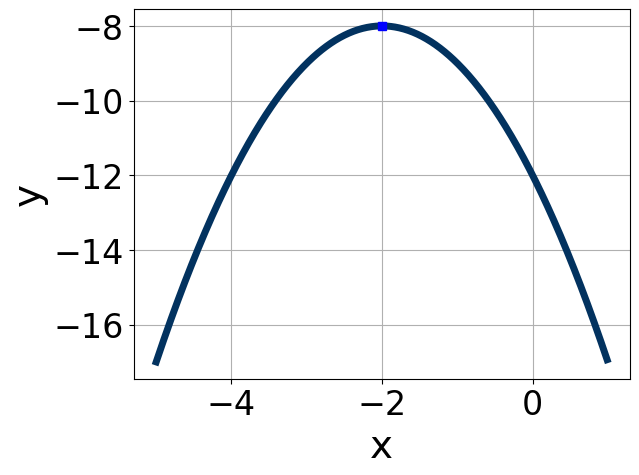
\includegraphics[width=0.5\textwidth]{../Figures/quadraticGraphToEquationB.png}
\end{center}
\begin{enumerate}[label=\Alph*.]
\item \( a \in [-0.1, 1.6], \hspace*{5mm} b \in [-7, -3], \text{ and } \hspace*{5mm} c \in [-4, -1] \)
\item \( a \in [-0.1, 1.6], \hspace*{5mm} b \in [3, 5], \text{ and } \hspace*{5mm} c \in [-4, -1] \)
\item \( a \in [-2.3, 0.7], \hspace*{5mm} b \in [3, 5], \text{ and } \hspace*{5mm} c \in [1, 6] \)
\item \( a \in [-2.3, 0.7], \hspace*{5mm} b \in [-7, -3], \text{ and } \hspace*{5mm} c \in [-12, -11] \)
\item \( a \in [-2.3, 0.7], \hspace*{5mm} b \in [3, 5], \text{ and } \hspace*{5mm} c \in [-12, -11] \)

\end{enumerate} }
\litem{
Solve the quadratic equation below. Then, choose the intervals that the solutions $x_1$ and $x_2$ belong to, with $x_1 \leq x_2$.\[ 25x^{2} -60 x + 36 = 0 \]\begin{enumerate}[label=\Alph*.]
\item \( x_1 \in [0.37, 0.5] \text{ and } x_2 \in [3.1, 5] \)
\item \( x_1 \in [29.95, 30.06] \text{ and } x_2 \in [28.7, 31.3] \)
\item \( x_1 \in [1.1, 1.58] \text{ and } x_2 \in [0.5, 1.8] \)
\item \( x_1 \in [0.08, 0.26] \text{ and } x_2 \in [3.9, 7.1] \)
\item \( x_1 \in [0.5, 0.95] \text{ and } x_2 \in [1.9, 3.4] \)

\end{enumerate} }
\litem{
Factor the quadratic below. Then, choose the intervals that contain the constants in the form $(ax+b)(cx+d); b \leq d.$\[ 36x^{2} -60 x + 25 \]\begin{enumerate}[label=\Alph*.]
\item \( a \in [0, 1.08], \hspace*{5mm} b \in [-31, -27], \hspace*{5mm} c \in [0.5, 1.4], \text{ and } \hspace*{5mm} d \in [-38, -28] \)
\item \( a \in [1.67, 3.14], \hspace*{5mm} b \in [-8, -1], \hspace*{5mm} c \in [9.1, 14.6], \text{ and } \hspace*{5mm} d \in [-10, -3] \)
\item \( a \in [11.14, 12.1], \hspace*{5mm} b \in [-8, -1], \hspace*{5mm} c \in [2.6, 4.8], \text{ and } \hspace*{5mm} d \in [-10, -3] \)
\item \( a \in [5.24, 6.79], \hspace*{5mm} b \in [-8, -1], \hspace*{5mm} c \in [3.7, 6.9], \text{ and } \hspace*{5mm} d \in [-10, -3] \)
\item \( \text{None of the above.} \)

\end{enumerate} }
\litem{
Write the equation of the graph presented below in the form $f(x)=ax^2+bx+c$, assuming  $a=1$ or $a=-1$. Then, choose the intervals that $a, b,$ and $c$ belong to.
\begin{center}
    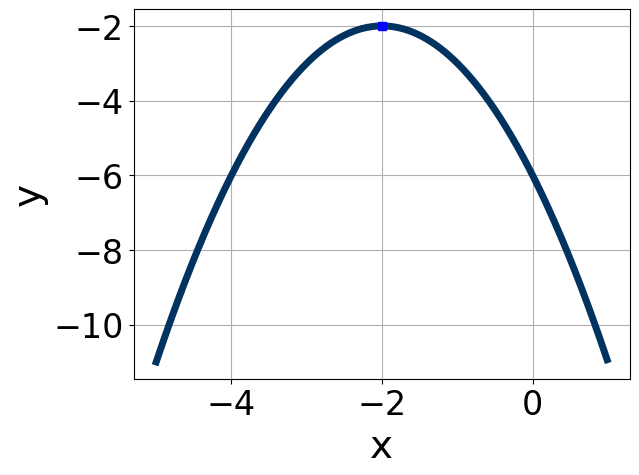
\includegraphics[width=0.5\textwidth]{../Figures/quadraticGraphToEquationCopyB.png}
\end{center}
\begin{enumerate}[label=\Alph*.]
\item \( a \in [-2, 0], \hspace*{5mm} b \in [1, 7], \text{ and } \hspace*{5mm} c \in [-7, -4] \)
\item \( a \in [1, 4], \hspace*{5mm} b \in [-6, -3], \text{ and } \hspace*{5mm} c \in [0, 5] \)
\item \( a \in [-2, 0], \hspace*{5mm} b \in [-6, -3], \text{ and } \hspace*{5mm} c \in [-7, -4] \)
\item \( a \in [-2, 0], \hspace*{5mm} b \in [1, 7], \text{ and } \hspace*{5mm} c \in [-2, 1] \)
\item \( a \in [1, 4], \hspace*{5mm} b \in [1, 7], \text{ and } \hspace*{5mm} c \in [0, 5] \)

\end{enumerate} }
\litem{
Solve the quadratic equation below. Then, choose the intervals that the solutions $x_1$ and $x_2$ belong to, with $x_1 \leq x_2$.\[ 25x^{2} +15 x -54 = 0 \]\begin{enumerate}[label=\Alph*.]
\item \( x_1 \in [-10.2, -8.91] \text{ and } x_2 \in [0.11, 0.33] \)
\item \( x_1 \in [-2.15, -0.9] \text{ and } x_2 \in [1.08, 2.44] \)
\item \( x_1 \in [-0.74, -0.47] \text{ and } x_2 \in [3.46, 4.1] \)
\item \( x_1 \in [-45.52, -42.96] \text{ and } x_2 \in [29.47, 30.44] \)
\item \( x_1 \in [-7.12, -4.54] \text{ and } x_2 \in [0.33, 0.57] \)

\end{enumerate} }
\end{enumerate}

\end{document}